\documentclass[a4paper, 10pt]{article}

\usepackage[utf8]{inputenc}
\usepackage{ amsmath, longtable, pgfplots, colortbl, float}
\usepackage[hidelinks]{hyperref}
\title{Predicting forset cover type from cartographic variables only}
\author{Cristian Di Pietrantonio}

\begin{document}

\maketitle
\begin{abstract}
This report has the objective to show how different classifiers perform on the forest cover type problem. In particular, Naive Bayes, Neural Network, Decision Tree and Random Forest are subject to accuracy testing, cross validation and learning curve analysis to establish which one is best suited to model the phenomenon. It will be discovered that ensem
\end{abstract}
\newpage
\tableofcontents
\newpage

\section{Introduction}

The objective of this work is to develop and compare different models of a phenomenon using machine learning techniques. In particular, the interest lays in predicting the forest cover type of a region given certain characteristics of the soil and the environment.

In order to do so, a large dataset of 581012 instances is provided, where each instance is an observation of a $30 \times 30$ meter cell characterized by 54 attributes and associated with the correct class of forest cover type. The 54 columns of data are divided as follows: 10 quantitative variables, 4 binary wilderness areas and 40 binary soil type variables.

It is thus a classification problem. To find the best model different machine learning algorithms are evaluated, each one with carefully selected parameters; next, a comparison of their predictive capacity (accuracy) and some other metrics takes place to find out which type of classifier best fit the problem to be solved. In particular, the following supervised learning algorithms are evaluated: \emph{Naive Bayes}, \emph{Neural Networks}, \emph{Decision Tree}, and \emph{Random Forest}. The choice has not been casual: each one of these classifiers works in a different way from the others, so that the probability of finding the best approach is maximized.

\section{Experimental settings and planning} 
In this section experimental settings, that are machines and tools used, are described. Furthermore, the experiments' structure will be laid out, indicating which set of tests classifiers are subject to in order to be evaluated.

\subsection{Hardware and software}
Experiments will be performed on a laptop having 12Gb og RAM DDR3, an Inter Core i7 processor with a maximum clock frequency of 3.4ghz and a Nvidia GeForce 820M GPU. 

On the software side, Python has been selected as programming language for its ease of use and the vast number of good machine learning libraries. In particular, the module implementing machine learning algorithms that has been chosen is \href{http://scikit-learn.org/}{scikit-learn}; it is the most used machine learning Python library in the scientific community, so it is well tested and optimized. Following the guidelines of Python, only few lines of code are needed to run a classifier in scikit-learn. The typical workflow is the following:
\begin{itemize}
	\item Initialize a new classifier object, for example a Multilayer Perceptron, passing the needed parameters to the constructor. Parameters are specific for each classifier.
	\begin{center}
		\fontfamily{pcr}\selectfont
		clf = MLPClassifier(hidden\_layer\_sizes=(25))
	\end{center}

	\item Fit the classifier using training data:
		\begin{center}
		\fontfamily{pcr}\selectfont
		clf.fit(feature\_vectors, labels)
		\end{center}
	
	\item Finally, give the classifier instance unseen instances and get a predicted label for them:
		\begin{center}
		\fontfamily{pcr}\selectfont
		predictions = clf.predict(unseen\_instances)
		\end{center}
\end{itemize}

Every classifier implements the \emph{fit} and \emph{predict} methods. Furthermore, scikit-learn has a lot of functions to manipulate data and perform testing and cross-validation.

Even though scikit-learn implements a lot of machine learning functions, a series of helper functions have been implemented in first person. For example, a class \emph{Dataset} has been created to deal with the dataset and it is capable of: computing the information gain; splitting the dataset randomly in $K$ subset of the same size; creating a subsample of the original dataset in such a way to keep the same class distribution (this is useful when testing different parameters without spending too much computation time on it).

\subsection{Experiment structure}
The final objective is to compare different classifiers, so it is mandatory that they all have to be subject to the same set of tests and evaluation criteria. The following phases are established:
\begin{enumerate}
 \item \emph{Preprocessing}: the dataset will be subject to a series of manipulations to make classifiers find an optimal fit more easily and in less time;
 \item For each classifier $C$:
 \begin{enumerate}
  
    \item \emph{Best parameters search}: given $C$, different values for its parameters will be tested in order to find a satisfying combination;
    \item \emph{Accuracy Testing}: the capabilities of classifier $C$ are first tested using a dataset split. More precisely, it is split in \emph{training} and \emph{test} set, the latter having $37\%$ of the instances in the original dataset;
    \item \emph{K-Fold Cross Validation}: the accuracy of classifier $C$ is assessed using K fold cross validation, with $K = 30$. In this way we can estimate the mean accuracy and its $95\%$ confidence interval;
    \item \emph{Learning curve}: as last test, accuracy is observed as a function of the dataset size. We can then recognize whether a classifier's performance depends heavily on the data quantity.
  \end{enumerate}
 \item \emph{Classifiers' performances comparison}: having gathered the data, a comparison takes place to establish which one can best fit the prediction task.
\end{enumerate}


\section{Preprocessing}
The first step involves data analysis and preprocessing. It is important to assess the quality and quantity of information contained in the dataset; these traits can influence and explain particular behaviors of a classifier. Moreover, data can be in a form not yet suitable for training a classifier, and must be manipulated to guarantee the best performances in terms of quality of prediction and time.

\subsection{Entropy and Class Distribution}
Entropy is a measure of uncertainty of a random variable. In this case the random variable is the class attribute in each example in the dataset. So it gives a measure of how much instances in this dataset are predictable. Entropy is computed using the following formula:
\begin{equation}
	\textit{Entropy} = \sum_{c \in C}\dfrac{n_c}{n}\log_2\left(\dfrac{n_c}{n}\right),
\end{equation}
Where $C$ is the set of labels (or classes) and $n_c$ is the number of instances belonging to class $c$. In our case entropy is equal to $1.73$ (the maximum value is $2.8$) or, equivalently, $61\%$. This means that instances are not equally distributed amongst classes. Considering the class attribute as a random variable, its distribution is shown in Table \ref{tab:class_dist}. To make more evident the disparity in class distribution, a bar chart with the probabilities is shown in Figure \ref{fig:class_dist}.  

\begin{table}[H]
 \centering
 \begin{tabular}{|l|l|}
 \hline
 \textbf{Class} & \textbf{Probability} \\\hline
 1 & 0.36461\\\hline
2 & 0.48760\\\hline 
3 & 0.06154\\\hline 
4 & 0.00473\\\hline 
5 & 0.01634\\\hline 
6 & 0.02989\\\hline
7 & 0.03530\\\hline
 \end{tabular}
\caption{class distribution.}
\label{tab:class_dist}
\end{table}

\begin{figure}[H]
 \centering
 \includegraphics[width=0.8\linewidth]{pictures/class_dist.eps}
 \caption{class distribution in a bar chart.}
 \label{fig:class_dist}
\end{figure}

Classes 1 and 2 hold most of the instances, followed by class 3. Class 4 has a very low frequency, so one can imagine that will be harder to learn to recognized it, in contrast with the first two. This dataset gives the possibility of studying classifiers' performances in non optimal conditions.

\subsection{Information Gain of Attributes}
To have an idea on how much each attribute contributes in determining the label of an example, \emph{information gain} of attribute $j$ is computed using the following formula:

\begin{equation}
	\textit{InformationGain} = \textit{Entropy} - \sum_{v \in \textit{V}_j}\dfrac{n_v}{n}\textit{Entropy}(S_v),
\end{equation}

where $S_v$ is the set of instances that have value $v$ for feature $j$. Information gain is computed over the dataset, for each attribute, and the results are shown in Table \ref{tab:infogain}.

\renewcommand{\arraystretch}{1.2}
\begin{longtable}{|l|l|l|}
	\hline
Attribute ID & Absolute value & Percentage value \\\hline
0 &  0.6662 &  38.32 \\\hline
13 &  0.2108 &  12.12 \\\hline
5 &  0.1513 &  8.70 \\\hline
9 &  0.1225 &  7.05 \\\hline
10 &  0.0962 &  5.53 \\\hline
23 &  0.0923 &  5.31 \\\hline
2 &  0.0526 &  3.02 \\\hline
6 &  0.0463 &  2.66 \\\hline
51 &  0.0440 &  2.53 \\\hline
42 &  0.0428 &  2.46 \\\hline
52 &  0.0419 &  2.41 \\\hline
17 &  0.0405 &  2.33 \\\hline
3 &  0.0367 &  2.11 \\\hline
35 &  0.0347 &  2.00 \\\hline
25 &  0.0344 &  1.98 \\\hline
15 &  0.0338 &  1.95 \\\hline
8 &  0.0325 &  1.87 \\\hline
7 &  0.0324 &  1.86 \\\hline
1 &  0.0316 &  1.82 \\\hline
36 &  0.0304 &  1.75 \\\hline
19 &  0.0288 &  1.66 \\\hline
4 &  0.0287 &  1.65 \\\hline
53 &  0.0255 &  1.47 \\\hline
16 &  0.0210 &  1.21 \\\hline
11 &  0.0192 &  1.10 \\\hline
14 &  0.0179 &  1.03 \\\hline
43 &  0.0167 &  0.96 \\\hline
26 &  0.0141 &  0.81 \\\hline
45 &  0.0128 &  0.73 \\\hline
46 &  0.0104 &  0.60 \\\hline
24 &  0.0103 &  0.59 \\\hline
12 &  0.0103 &  0.59 \\\hline
30 &  0.0095 &  0.55 \\\hline
18 &  0.0094 &  0.54 \\\hline
44 &  0.0076 &  0.43 \\\hline
37 &  0.0072 &  0.41 \\\hline
48 &  0.0069 &  0.39 \\\hline
27 &  0.0043 &  0.24 \\\hline
31 &  0.0027 &  0.16 \\\hline
33 &  0.0026 &  0.15 \\\hline
50 &  0.0025 &  0.14 \\\hline
39 &  0.0025 &  0.14 \\\hline
32 &  0.0021 &  0.12 \\\hline
34 &  0.0018 &  0.10 \\\hline
47 &  0.0016 &  0.09 \\\hline
41 &  0.0012 &  0.07 \\\hline
22 &  0.0010 &  0.06 \\\hline
29 &  0.0009 &  0.05 \\\hline
40 &  0.0004 &  0.03 \\\hline
49 &  0.0004 &  0.02 \\\hline
38 &  0.0003 &  0.01 \\\hline
20 &  0.0002 &  0.01 \\\hline
21 &  0.0001 &  0.01 \\\hline
28 &  0.0000 &  0.00 \\\hline
\caption{Attributes ranked by Information Gain.}
\label{tab:infogain}
\end{longtable}

The first two attributes, namely \emph{Elevation} and a binary column of the abstract attribute \emph{Wilderness Area}. At the opposite side, we have the $28^{\textit{th}}$ attribute that has no influence on class distribution. In order to make computations faster, attributes with information gain less than $0.1\%$ are removed (9 attributes).

Next, quantitative attributes are normalized to speed up computation (for example, a gradient descent algorithm could take a significant amount of time to converge if the range of values is large) and to give each attribute equal weight in distance-based machine learning algorithms (k-means, for example).

Here ends the preprocessing work done on the dataset. All other attributes take binary values so there is nothing that can be done to reach noticeable better performances.

\section{Naive Bayes}

The first classifier to be tested is Naive Bayes. A Naive Bayes classifier assumes the independence of the components in the feature vector and compute the probability $P(y_i | \mathbf{x})$ of label $y_i$ given the observed instance $\mathbf{x}$ using Bayes' theorem:
\begin{equation}
 P(y_i | \mathbf{x}) = \dfrac{P(y_i)P(\mathbf{x} | y_i)}{P(\mathbf{x})}  = \dfrac{P(y_i)\prod_{j=1}^nP(X_j = v_{jk}|Y = y_i)}{P(\mathbf{x})},
\end{equation}

with $i = 1,\ldots, m$, where $n$ is the number of features, $m$ the number of examples. The theorem allows us to compute needed probabilities from the dataset. For this classifier, two experiments will be performed: in the first it is assumed that the features underlying distribution is Gaussian, in the second a multinomial one.

As for the parameters tuning, the only ones that can be set are the \emph{priors}. It has been decided to apply Laplace Smoothing, which is the default option and a reasonable one.

\subsection{Gaussian Naive Bayes}

Since some features take on real values one can think that their underlying distribution is Gaussian and mean and variance can be estimated for feature $X_j$ given that the example belongs to class $y_i$. Then, the probability of each feature value is computed using the following formula:

\begin{equation}
 P(X_j = v_{jk}|Y = y_i) = \dfrac{1}{\sigma_{ji}\sqrt{2\pi}}\textit{exp}\left(\dfrac{-(X_j - \mu_{ji})^2}{2\sigma^2_{ji}}\right)
\end{equation}

\subsubsection{Accuracy Testing}

A first test is run to assess classifier's capacity using a dataset split, training the model with $63\%$ of the data and testing it with the remaining instances. The resulting accuracy is equal to $17.40\%$ or, equivalently, the error is equal to $82.6\%$. It is clear that the current classifier performs very poorly with this dataset. Table \ref{tab:gnb_test_pr} shows detailed statistics for each class; Table \ref{tab:gnb_cf} shows the confusion matrix. As can be seen we have high precision on the classes (1 and 2) having the major number of instances, but recall capacity is really low. This suggests that lack of equidistribution have played an important role in causing poor performances.

\begin{table}[H]
\centering
\begin{tabular}{|l|l|l|l|}
\hline
\textbf{Class Index} & \textbf{Precision} & \textbf{Recall} & \textbf{F-Measure}\\\hline
1 & 69.830 & 14.093& 23.453\\\hline
2 & 90.310 & 9.601& 17.356\\\hline
3 & 27.364 & 39.720& 32.404\\\hline
4 & 7.557 & 100.000& 14.051\\\hline
5 & 2.431 & 71.957& 4.702\\\hline
6 & 18.282 & 6.362& 9.439\\\hline
7 & 14.648 & 93.715& 25.335\\\hline
\end{tabular}
\caption{precision and recall for each class.}
\label{tab:gnb_test_pr}
\end{table}



\begin{table}[H]
\centering
\begin{tabular}{|*{7}{c|}r|}
\hline

1 &2 &3 &4 &5 &6 &7 & $\leftarrow$ classified as \\\hline

\cellcolor{black!15}14.09 &1.37 &1.31 &0.00 &46.49 &0.95 &35.80 & 1 \\\hline

4.49 &\cellcolor{black!15}9.60 &9.40 &1.06 &62.17 &1.01 &12.27 & 2 \\\hline

0.00 &0.00 &\cellcolor{black!15}39.72 &59.67 &0.45 &0.17 &0.00 & 3 \\\hline

0.00 &0.00 &0.00 &\cellcolor{black!15}100.00 &0.00 &0.00 &0.00 & 4 \\\hline

0.17 &0.00 &26.43 &0.00 &\cellcolor{black!15}71.96 &0.82 &0.62 & 5 \\\hline

0.39 &0.00 &32.02 &55.87 &5.11 &\cellcolor{black!15}6.36 &0.25 & 6 \\\hline

0.79 &0.00 &1.00 &0.00 &4.50 &0.00 &\cellcolor{black!15}93.72 & 7 \\\hline

\end{tabular}
\caption{Confusion matrix for Gaussian Naive Bayes.}
\label{tab:gnb_cf}
\end{table}


\subsubsection{Cross Validation}
The next step is to apply K-fold cross validation, with $K=30$, to assess the classifier's performance with reasonably confidence in what will be discovered. Accuracy in each trial (fold) is computed and the resulting mean accuracy is $17.468\%$, with a $95\%$ confidence interval of $\pm 0.110$. 

As can be seen in Figure \ref{fig:acc_int_gnb}, in each fold the classifier has a very low accuracy. This explains why the confidence interval is small around the mean. Cross validation confirmed what was saw before: Naive Bayes, with the Gaussian assumption, is unable to predict the cover type. Furthermore, precision, recall and f-measure of each class, shown in Table \ref{tab:gnb_pr} and Figure \ref{fig:gnb_fmeasure}, show a great unbalance between precision and recall. Classes 3 has the highest \emph{harmonic mean} (that is, F-measure), while on class 4 the classifier shows full recall capability (this may be due to the fact that there are really few class 4 instances). Overall, F-measure values are really low, confirming that this classifier would be a poor choice.

\begin{figure}[H]
 \centering
 \includegraphics[width=0.8\linewidth]{pictures/nb_gaussian_accuracy_interval.eps}
 \caption{Mean accuracy and confidence interval for Gaussian Naive Bayes.}
 \label{fig:acc_int_gnb}
\end{figure}

\begin{table}[H]
\centering
\begin{tabular}{|l|l|l|l|}
\hline
\textbf{Class Index} & \textbf{Precision} & \textbf{Recall} & \textbf{F-Measure}\\\hline
1 & 69.276 & 14.120& 23.456\\\hline
2 & 90.805 & 9.628& 17.409\\\hline
3 & 27.295 & 39.456& 32.260\\\hline
4 & 7.430 & 100.000& 13.819\\\hline
5 & 2.512 & 74.007& 4.859\\\hline
6 & 14.758 & 6.656& 9.161\\\hline
7 & 14.634 & 93.974& 25.320\\\hline
\end{tabular}
\caption{mean precision, recall and F-measure using cross validation.}
\label{tab:gnb_pr}
\end{table}

\begin{figure}[H]
 \centering
 \includegraphics[width=0.8\linewidth]{pictures/nb_gaussian_fmeasure.eps}
 \caption{F-measures resulting from cross validation.}
 \label{fig:gnb_fmeasure}
\end{figure}


\subsubsection{Learning curve}

\begin{table}[H]
\centering
\begin{tabular}{|l|l|}
\hline
\textbf{Dataset Size} & \textbf{Accuracy}\\\hline
58102 & 12.350\\\hline
116203 & 12.966\\\hline
174304 & 12.639\\\hline
232405 & 17.330\\\hline
290506 & 17.266\\\hline
348607 & 17.525\\\hline
406708 & 17.525\\\hline
464809 & 17.537\\\hline
522910 & 17.536\\\hline
581011 & 17.473\\\hline
\end{tabular}
\caption{Dataset sizes and relative accuracy.}
\label{tab:gnb_learning}
\end{table}

As final test, the learning curve of the classifier is studied. The main dataset is divided in ten parts and another ten datasets, of growing size, are created. Can the classifier improve its performance with a lager set of data? To answer this question, Naive Bayes is tested on the newly created datasets, and every accuracy value is annotated in Table \ref{tab:gnb_learning}. The minimum value is $12.3$, associated with the smallest dataset; the maximum value is $17.537$, obtained using one of the largest dataset. It can be said that there has been an improvement, even though a small one considering the datasets' size. Looking at Figure \ref{fig:gnb_learning} it is clear that size $200k$ acts as the threshold for improvement. The first three points are stable around $12.5$; then there is a jump to $17.3$ and from that point on the learning curve becomes flat at that value. It follows that most likely a greater dataset cannot improve the classifier's performance.

\begin{figure}[H]
 \centering
 \includegraphics[width=0.8\linewidth]{pictures/nb_gaussian_size_vs_accuracy.eps}
 \caption{Learning curve of Gaussian Naive Bayes.}
 \label{fig:gnb_learning}
\end{figure}

    
\subsection{Multinomial Naive Bayes}

Now the distribution assumption on features' values is changed to a multinomial one. Feature vectors represent the frequencies with which features have been observed and are modeled by a multinomial distribution.

\subsubsection{Accuracy Testing}
As before, the dataset is split in test set and training set; a multinomial Naive Bayes classifier instance is run. The accuracy registered is equal to $64.013\%$ and, even though it is not a good enough value, it shows a huge improvement in performance with respect to the Gaussian Naive Bayes classifier. Detailed statistics are listed in Table \ref{tab:mnb_test_pr}. Table \ref{tab:mnb_cf} shows the confusion matrix. The first thing to be noticed is that class 5 is not recognized at all; in the case of the Gaussian distribution, it had the lowest F-measure, $4.8$, and it is the second lowest frequent class in the dataset. Most of class 5 instances are classified as belonging to class 2, as can be seen in the confusion matrix. Class 4 and 6 are still hard to recognize, in fact a lot of their instances are misclassified with label 3. On the other hand, all the other classes present higher values for both precision and recall, and these values are balanced.

\begin{table}[H]
\centering
\begin{tabular}{|l|l|l|l|}
\hline
\textbf{Class Index} & \textbf{Precision} & \textbf{Recall} & \textbf{F-Measure}\\\hline
1 & 65.315 & 46.433& 54.278\\\hline
2 & 64.730 & 80.886& 71.912\\\hline
3 & 55.646 & 92.842& 69.585\\\hline
4 & 65.730 & 11.448& 19.500\\\hline
5 & 0.000 & 0.000& 0.000\\\hline
6 & 43.750 & 2.615& 4.935\\\hline
7 & 68.483 & 49.605& 57.535\\\hline
\end{tabular}
\caption{precision, recall and f-measure of classes using multinomial Naive Bayes.}
\label{tab:mnb_test_pr}
\end{table}


\begin{table}[H]
\centering
\begin{tabular}{|*{7}{c|}r|}
\hline

1 &2 &3 &4 &5 &6 &7 & $\leftarrow$ classified as \\\hline

\cellcolor{black!15}46.43 &51.38 &0.11 &0.00 &0.00 &0.00 &2.08 & 1 \\\hline

15.32 &\cellcolor{black!15}80.89 &3.66 &0.00 &0.00 &0.00 &0.13 & 2 \\\hline

0.00 &5.96 &\cellcolor{black!15}92.84 &0.42 &0.00 &0.78 &0.00 & 3 \\\hline

0.00 &0.00 &77.89 &\cellcolor{black!15}11.45 &0.00 &10.67 &0.00 & 4 \\\hline

8.14 &82.18 &9.67 &0.00 &\cellcolor{black!15}0.00 &0.00 &0.00 & 5 \\\hline

0.90 &23.99 &72.43 &0.06 &0.00 &\cellcolor{black!15}2.62 &0.00 & 6 \\\hline

36.33 &13.64 &0.43 &0.00 &0.00 &0.00 &\cellcolor{black!15}49.61 & 7 \\\hline

\end{tabular}
\caption{confusion matrix for multinomial Naive Bayes.}
\label{tab:mnb_cf}
\end{table}

\subsubsection{Cross validation}
It is now the moment to apply cross validation. The mean accuracy obtained is $64.165\%$, with a $95\%$ confidence interval of $\pm0.103$, shown in Figure \ref{fig:acc_int_mnb}. This result is in accordance with what has been found in the previous test. The small confidence interval indicates that the sample mean value is indeed representative of the true accuracy of the classifier. As has already been said, $64\%$ is still a non satisfactory value, but represents a great improvement to the Gaussian classifier's one. Detailed statistics for each class are shown in Table \ref{tab:mnb_cross_pr}. Even in cross validation class 5 is still not recognized, while other classes present a precision percentage around $60\%$. Recall values are more sparse, going from $2.4\%$ to $92.9\%$ (excluding class 5). F-Measure values, as can be seen also in Figure \ref{fig:mnb_fmeasure}, are fairly high for classes 1, 2, 3 and 7. It is interesting to note that class 7 has a relatively high f-measure, even though its instances are not frequent in the dataset, with respect to class 1 and 2 instances; yet, they present approximately the same F-measure. It may be that exist feature values particular to that class of instances. 

\begin{figure}[H]
 \centering
 \includegraphics[width=0.8\linewidth]{pictures/nb_multi_accuracy_interval.eps}
 \caption{Mean accuracy and confidence interval for Gaussian Naive Bayes.}
 \label{fig:acc_int_mnb}
\end{figure}

\begin{table}[H]
\centering
\begin{tabular}{|l|l|l|l|}
\hline
\textbf{Class Index} & \textbf{Precision} & \textbf{Recall} & \textbf{F-Measure}\\\hline
1 & 66.014 & 46.460& 54.536\\\hline
2 & 64.665 & 80.939& 71.892\\\hline
3 & 55.770 & 92.988& 69.716\\\hline
4 & 67.020 & 12.332& 20.686\\\hline
5 & 0.000 & 0.000& 0.000\\\hline
6 & 46.617 & 2.483& 4.710\\\hline
7 & 68.271 & 53.977& 60.265\\\hline
\end{tabular}
\caption{mean precision, recall, F-measure for multinomial Naive Bayes in cross validation.}
\label{tab:mnb_cross_pr}
\end{table}
\begin{figure}[H]
 \centering
 \includegraphics[width=0.8\linewidth]{pictures/nb_multi_fmeasure.eps}
 \caption{F-measure of classes resulting from cross validation.}
 \label{fig:mnb_fmeasure}
\end{figure}


\subsubsection{Learning curve}
The classifier's accuracy has been evaluated over different dataset sizes and results are shown in Table \ref{tab:mnb_learning}; the learning curve for multinomial Naive Bayes classifier is shown in Figure \ref{fig:mnb_learning}. In this case accuracy seems to be independent from the dataset size, since it is stable at $64\%$.

\begin{table}[H]
\centering
\begin{tabular}{|l|l|}
\hline
\textbf{Dataset Size} & \textbf{Accuracy}\\\hline
58102 & 64.536\\\hline
116203 & 64.041\\\hline
174304 & 64.114\\\hline
232405 & 64.504\\\hline
290506 & 64.086\\\hline
348607 & 64.055\\\hline
406708 & 64.075\\\hline
464809 & 64.168\\\hline
522910 & 64.185\\\hline
581011 & 64.266\\\hline
\end{tabular}
\caption{Dataset sizes and relative accuracy for multinomial Naive Bayes.}
\label{tab:mnb_learning}
\end{table}

\begin{figure}[H]
 \centering
 \includegraphics[width=0.8\linewidth]{pictures/nb_multi_size_vs_accuracy.eps}
 \caption{Learning curve for multinomial Naive Bayes.}
 \label{fig:mnb_learning}
\end{figure}


  
\section{Neural Networks}
Neural networks are a computational approach that loosely model the way biological brain solves problems. The model is composed by several units, called \emph{perceptrons}, organized in multiple \emph{layers}, where each unit in layer $i$ is \emph{activated} when receiving a \emph{signal} from all the units in layer $i-1$. The first layer represent the input vector, the last layer encodes the output. There is a weight on each edge connecting two perceptrons, which proportionally amplify the signal on that edge. The problem is to find a set of weights that make a neural network predict the right output for a given input vector.

\subsection{Parameters selection}
The first decision to take when using neural networks to solve a problem regards its architecture. In particular the number of \emph{hidden layers} and the number of perceptrons in each layer must be defined. Since we will use the backpropagation algorithm, the number of hidden layers suggested in literature is one. Since the number of input units and output units is fixed, it remains to decide how many hidden units are needed. What has been done is defining a search space and try every value in it, using a \emph{subsample} of the original dataset (the reason is to avoid too long computation time just for parameter tuning). Another parameter to be chosen is the maximum number of \emph{epochs} that a neural network goes through during the training phase: $300$ is considered a reasonable value given the size of the dataset.

The search space defined is $$\mathcal{S} = \{10, 15, 18, 20, 23, 25, 27, 30, 35, 40, 45\}$$ that is, numbers between $n$ and $\sqrt{n}$, where $n$ is the number of features. As for the subsample, an apposite function was manually implemented to pick a set of instances of a given size from the original dataset such that the distribution of class values does not change. In this case, the subsample contain $5\%$ of the original number of instances (which is still a great number of instances, $29000$).

For each value in $\mathcal{S}$ we build a neural network with that number of hidden units and test it with 5-fold cross validation. The number of hidden units associated with the highest score is chosen.

\begin{figure}[H]
 \centering
 \includegraphics[width=0.8\linewidth]{pictures/nn_hidden_units.eps}
 \caption{Scores obtained variating the number of hidden units in a neural network.}
 \label{fig:nn_hidden_units}
\end{figure}

As can be seen in Figure \ref{fig:nn_hidden_units}, in general the more hidden units more is the score obtained. The highest score is associated with $40$ hidden units, so that values is chosen by the automated script that performs the various tests. It is to be noticed that the improvement in accuracy is not noticeable so a smaller number of hidden units would have been fine (it is also true that these results are valid on the \emph{subsample}; maybe a major number of hidden units is needed to handle the original dataset well).

\subsection{Accuracy Testing}
Now that parameters has been chosen, in order to have a general idea of its capabilities, the neural network is trained using $63\%$ of the instances in the dataset and tested using the remaining $37\%$. The accuracy of the neural network is $79.908\%$, which is a decent value, considering the non optimal distribution of instances in the various classes.

\begin{table}[H]
\centering
\begin{tabular}{|l|l|l|l|}
\hline
\textbf{Class Index} & \textbf{Precision} & \textbf{Recall} & \textbf{F-Measure}\\\hline
1 & 79.740 & 77.211& 78.455\\\hline
2 & 80.909 & 84.891& 82.852\\\hline
3 & 78.992 & 82.563& 80.738\\\hline
4 & 80.159 & 64.952& 71.758\\\hline
5 & 64.633 & 27.739& 38.818\\\hline
6 & 66.850 & 56.574& 61.285\\\hline
7 & 81.194 & 80.285& 80.737\\\hline
\end{tabular}
\caption{precision, recall and F-measure of classes using a neural network.}
\label{tab:nn_test_pr}
\end{table}

Table \ref{tab:nn_test_pr} shows detailed stats for each class. Precision values are quite good for all classes, with the maximum precision registered being $81\%$ and minimum $64\%$. As for recall, its values are still quite different from each other but in general are better than what has been seen so far. 

\begin{table}[H]
\centering
\begin{tabular}{|*{7}{c|}r|}
\hline

1 &2 &3 &4 &5 &6 &7 & $\leftarrow$ classified as \\\hline

\cellcolor{black!15}77.21 &20.98 &0.05 &0.00 &0.13 &0.03 &1.60 & 1 \\\hline

13.18 &\cellcolor{black!15}84.89 &0.80 &0.00 &0.41 &0.58 &0.14 & 2 \\\hline

0.00 &8.55 &\cellcolor{black!15}82.56 &0.88 &0.08 &7.93 &0.00 & 3 \\\hline

0.00 &0.00 &25.29 &\cellcolor{black!15}64.95 &0.00 &9.75 &0.00 & 4 \\\hline

6.22 &62.60 &2.68 &0.00 &\cellcolor{black!15}27.74 &0.76 &0.00 & 5 \\\hline

0.03 &16.55 &26.38 &0.45 &0.02 &\cellcolor{black!15}56.57 &0.00 & 6 \\\hline

17.69 &2.02 &0.00 &0.00 &0.00 &0.00 &\cellcolor{black!15}80.29 & 7 \\\hline

\end{tabular}
\caption{confusion matrix associated to neural network testing.}
\label{tab:nn_cf}
\end{table}

The resulting confusion matrix is shown in Table \ref{tab:nn_cf}. We can see that instances of class 5 are still hard to recognize (as when using Naive Bayes), while classes 1,2,3 and 7 are classified correctly most of the time. The classifier is weaker on class 4 and 6, but can be considered a decent result in light of the small number of examples at its disposal. 

\subsection{Cross validation}

To find out if $79.9\%$ is a value for accuracy to be confident with, cross validation is executed. The resulting mean accuracy is $80.033\%$, with a $95\%$ confidence interval of $\pm  0.274$. Mean precision is $77.139\%$, mean recall is $67.837\%$ and mean F-measure $70.848\%$. Also in this case, the cross validation indicates a mean accuracy which is nearly identical to the one in accuracy testing; furthermore, the confidence interval is small enough to guarantee that such value is very plausible. It can be seen in Figure \ref{fig:nn_accuracy_interval} accuracies of each fold keep themselves quite near the mean with only a few of them noticeably far from it. Table \ref{tab:nn_cross_pr} looks similar to Table \ref{tab:nn_test_pr}, the one in accuracy testing, with a low recall value only for instances of class 5.

\begin{figure}[H]
 \centering
 \includegraphics[width=0.8\linewidth]{pictures/nn_accuracy_interval.eps}
 \caption{Scores obtained variating the number of hidden units in a neural network.}
 \label{fig:nn_accuracy_interval}
\end{figure}

\begin{table}[H]
\centering
\begin{tabular}{|l|l|l|l|}
\hline
\textbf{Class Index} & \textbf{Precision} & \textbf{Recall} & \textbf{F-Measure}\\\hline
1 & 79.744 & 77.588& 78.556\\\hline
2 & 81.134 & 84.981& 82.963\\\hline
3 & 78.641 & 84.546& 81.423\\\hline
4 & 81.413 & 69.292& 74.716\\\hline
5 & 68.007 & 27.227& 38.370\\\hline
6 & 66.303 & 53.938& 59.130\\\hline
7 & 84.729 & 77.285& 80.773\\\hline
\end{tabular}
\caption{precision, recall and F-measure values resulting from cross validation.}
\label{tab:nn_cross_pr}
\end{table}

Plotting the F-measure values results in Figure \ref{fig:nn_fmeasure}. As the bar chart shows, all classes except 5 present a high valued harmonic mean between precision and recall, around $80\%$. This confirms that neural networks are a powerful tool that can be used to achieve decent results in classification problems involving complex phenomena or a non optimal class distribution.

\begin{figure}[H]
 \centering
 \includegraphics[width=0.8\linewidth]{pictures/nn_fmeasure.eps}
 \caption{F-measure scores obtained using a neural network.}
 \label{fig:nn_fmeasure}
\end{figure}


\subsection{Learning curve}

\begin{table}[H]
\centering
\begin{tabular}{|l|l|}
\hline
\textbf{Dataset Size} & \textbf{Accuracy}\\\hline
58102 & 75.728\\\hline
116203 & 76.140\\\hline
174304 & 77.256\\\hline
232405 & 78.099\\\hline
290506 & 78.403\\\hline
348607 & 79.264\\\hline
406708 & 78.510\\\hline
464809 & 78.318\\\hline
522910 & 79.739\\\hline
581011 & 80.050\\\hline
\end{tabular}
\caption{datasets size and relative accuracy using a neural network.}
\label{tab:nn_learning}
\end{table}

The last thing to understand about neural networks applied to the forest cover type problem is whether more data would have been helpful to achieve a better accuracy. The neural network is tested on the usual ten datasets of different size, Table \ref{tab:nn_learning} shows the collected values. At the beginning, with the smallest dataset,  the accuracy is around $75\%$; then, the more instances are in the dataset, more accuracy grows. For the first time a quite noticeable linear dependency between dataset size and accuracy is observed, as can be seen in Figure \ref{fig:nn_learning}. At the end an $80\%$ of accuracy is reached, that is, a $5\%$ increment.

\begin{figure}[H]
 \centering
 \includegraphics[width=0.8\linewidth]{pictures/nn_size_vs_accuracy.eps}
 \caption{Learning curve for neural network.}
 \label{fig:nn_learning}
\end{figure}

\section{Decision Tree}

A decision tree is tool that uses a tree graph to model decisions and possible consequences. It is used in machine learning to find features-based rules according to which observations about an instance (represented in internal nodes) are mapped to a target class (the leaves). Decision Tree Learning works by recursively splitting the training set according to a chosen feature and its values; the choice of feature to split data in an internal node in the tree is crucial. Most popular characteristics observed to make the decision are \emph{information gain}, that measures the quantity of information that a given feature carries and that is helpful in determining the label of the example, and \emph{Gini impurity}, that is a measure of how often a randomly chosen element from the set would be incorrectly labeled if it was randomly labeled according to the distribution of labels in the subset.

\subsection{Parameters selection}

In this subsection the most important parameters configurations are analyzed. The decision tree implementation in scikit-learn, the Python library used, the most important parameters that can be set are:
\begin{itemize}
 \item \emph{criterion}: the criterion that feature at an internal node is chosen with. Possible values are ``gini'', for Gini impurity, and ``entropy'', for Information Gain;
 \item \emph{max\_features}: the number of features to consider when looking for the best split. Tested values are $\{10, 15, 30, 35, 40\}$.
 \item \emph{min\_samples\_split}: the minimum number of examples required to split an internal node. Tested values are $\{2, 5, 10, 30, 50\}$.
 \item \emph{min\_samples\_leaf}: the minimum number of examples required to be a leaf node. Tested values are $\{5, 7, 15, 20, 50\}$.
\end{itemize}

The number of all configurations tested is $250$. To perform the search, also in this case a subsample containing $7\%$ of the original instances is used to speed up the operation. Figure \ref{fig:dt_config} shows the score as a function of the configuration tested.

\begin{figure}[H]
 \centering
 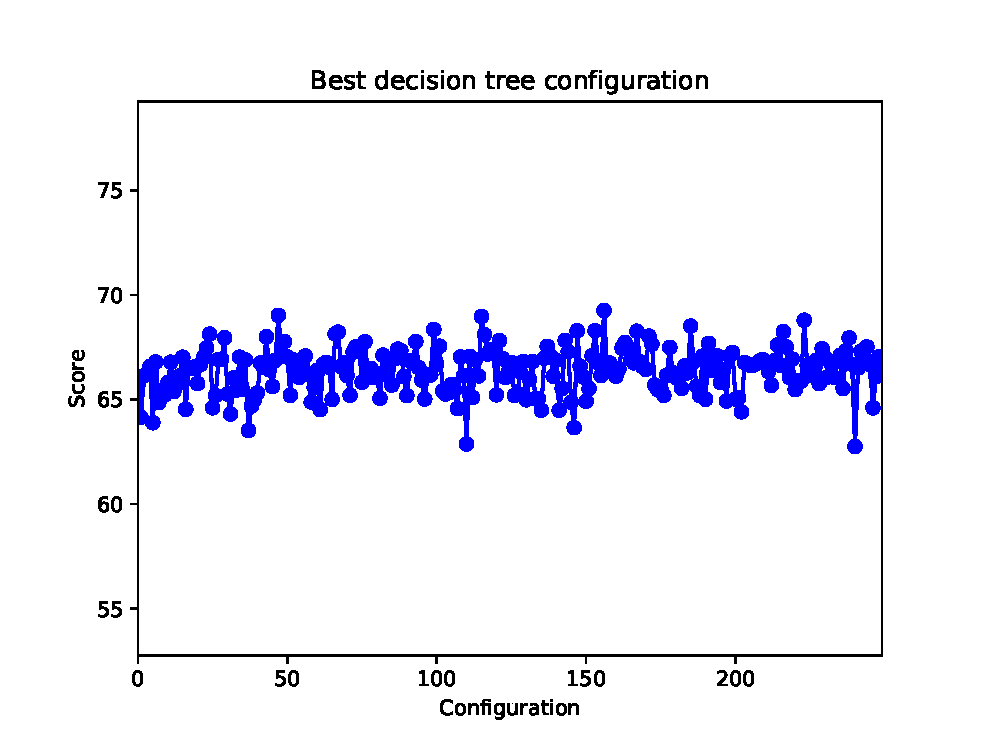
\includegraphics[width=0.8\linewidth]{pictures/decision_tree_config.eps}
 \caption{Optimal configuration search for decision tree.}
 \label{fig:dt_config}
\end{figure}

The best score registered is $69\%$ with \emph{criterion} ``gini'', \emph{min\_samples\_split} equal to 50, \emph{max\_features} equal to 15 and \emph{min\_samples\_leaf} equal to 15. The choice of this configuration has brought a $5\%$ improvement in accuracy according to this test. 
 
 
\subsection{Accuracy Testing}

The decision tree classifier instance created with parameters found in precedence is run using the full dataset, with the usual $37\%$ split for the test set. Its accuracy is equal to $86.864\%$, demonstrating that decision trees can be used to obtain pretty good results on the current classification problem. Now the attention is focused on precision and recall values for each class, shown in in Table \ref{tab:dt_test_pr}. Decision trees seems to fit well in predicting the forest cover type, since precision and recall values are quite high, with maximum precision and recall registered equal to $89\%$. There is not too much distance between precision and recall values, in fact most F-measures values are noticeably over the $70\%$ threshold. Table \ref{tab:dt_cm} shows the confusion matrix. Few misclassification problems are noticeable. Class 5 is recognized $55\%$ of the times, while $35\%$ of its instances are misclassified as belonging to class $2$. In the case of class 4, $23\%$ of its instances are classified as belonging to class 3. $19\%$ of instances of class 6 are labeled with $3$. Other values outside the diagonal are pretty low, so one can deduce that this classifier has the potential to handle the prediction task at hand. 
 
\begin{table}[H]
\centering
\begin{tabular}{|l|l|l|l|}
\hline
\textbf{Class Index} & \textbf{Precision} & \textbf{Recall} & \textbf{F-Measure}\\\hline
1 & 86.863 & 86.379& 86.620\\\hline
2 & 88.315 & 89.741& 89.023\\\hline
3 & 83.586 & 86.391& 84.965\\\hline
4 & 75.492 & 70.697& 73.016\\\hline
5 & 71.246 & 55.524& 62.410\\\hline
6 & 74.338 & 69.098& 71.622\\\hline
7 & 89.644 & 84.911& 87.213\\\hline
\end{tabular}
\caption{precision, recall, F-measure for decision tree.}
\label{tab:dt_test_pr}
\end{table}


\begin{table}[H]
\centering
\begin{tabular}{|*{7}{c|}r|}
\hline

1 &2 &3 &4 &5 &6 &7 & $\leftarrow$ classified as \\\hline

\cellcolor{black!15}86.38 &12.45 &0.01 &0.00 &0.23 &0.05 &0.87 & 1 \\\hline

8.53 &\cellcolor{black!15}89.74 &0.68 &0.01 &0.53 &0.45 &0.06 & 2 \\\hline

0.14 &4.92 &\cellcolor{black!15}86.39 &1.14 &0.24 &7.17 &0.00 & 3 \\\hline

0.00 &0.31 &23.67 &\cellcolor{black!15}70.70 &0.00 &5.33 &0.00 & 4 \\\hline

7.10 &35.08 &1.39 &0.00 &\cellcolor{black!15}55.52 &0.91 &0.00 & 5 \\\hline

0.49 &9.82 &19.31 &1.00 &0.28 &\cellcolor{black!15}69.10 &0.00 & 6 \\\hline

13.46 &1.59 &0.00 &0.00 &0.04 &0.00 &\cellcolor{black!15}84.91 & 7 \\\hline

\end{tabular}
\caption{confusion matrix of the decision tree.}
\label{tab:dt_cm}
\end{table}

\subsection{Cross validation}

Cross validation is performed to validate the decision tree instance used in accuracy testing. The resulting mean accuracy is $88.504\%$, with a $95\%$ confidence interval of $\pm 0.115$. Mean precision is $83.836\%$, recall is $80.546\%$ and F-measure is equal to $82.049\%$. It is an even better result than what has been obtained in accuracy testing. Figure \ref{fig:dt_accuracy} shows the confidence interval for accuracy computed using the accuracies of each fold. The maximum accuracy registered is around $89\%$, while the lowest is $87.8\%$; a difference of $1.2\%$ that is small enough to explain the tight confidence interval around the mean. Table \ref{tab:dt_cross_pr} shows precision, recall and f-measure values for each class. Precision and recall values are high, with class 7 having the maximum precision registered, $90\%$, and class 2 having the maximum recall registered, $90.8\%$. Class 5, the one most difficult to recognize, has decent precision and recall values.

\begin{figure}[H]
 \centering
 \includegraphics[width=0.8\linewidth]{pictures/decision_tree_accuracy_interval.eps}
 \caption{Accuracy interval for decision tree.}
 \label{fig:dt_accuracy}
\end{figure}

\begin{table}[H]
\centering
\begin{tabular}{|l|l|l|l|}
\hline
\textbf{Class Index} & \textbf{Precision} & \textbf{Recall} & \textbf{F-Measure}\\\hline
1 & 88.444 & 88.043& 88.242\\\hline
2 & 89.768 & 90.864& 90.312\\\hline
3 & 86.364 & 88.400& 87.365\\\hline
4 & 79.202 & 72.558& 75.601\\\hline
5 & 74.595 & 62.550& 67.987\\\hline
6 & 78.429 & 74.835& 76.568\\\hline
7 & 90.054 & 86.572& 88.267\\\hline
\end{tabular}
\caption{precision, recall and F-measure values resulting from decision tree.}
\label{tab:dt_cross_pr}
\end{table}

Figure \ref{fig:dt_fmeasure} shows graphically the F-measure values for each class. All the values are above $67\%$, with class 2 touching $90\%$. It follows that decision tree can indeed be a good classifier to use in this context.

\begin{figure}[H]
 \centering
 \includegraphics[width=0.8\linewidth]{pictures/decision_tree_fmeasure.eps}
 \caption{F-measure values for decision tree.}
 \label{fig:dt_fmeasure}
\end{figure}

 \subsection{Learning curve}
Now the learning curve will be plotted and analyzed. To do so, various accuracies relative to different datasets with different sizes are collected in Table \ref{tab:dt_learning}. The accuracy relative to the smallest dataset is $76\%$, and the one relative to the greatest is $86\%$. It is a remarkable $10\%$ increment in performance, that makes think about the possibility of even better performances with an greater dataset. Figure \ref{fig:dt_learning} shows this increment in a graphical way.
\begin{table}[H]
\centering
\begin{tabular}{|l|l|}
\hline
\textbf{Dataset Size} & \textbf{Accuracy}\\\hline
58102 & 76.854\\\hline
116203 & 79.703\\\hline
174304 & 82.356\\\hline
232405 & 82.532\\\hline
290506 & 83.542\\\hline
348607 & 84.368\\\hline
406708 & 85.017\\\hline
464809 & 85.746\\\hline
522910 & 85.980\\\hline
581011 & 86.327\\\hline
\end{tabular}
\caption{Datasets size and relative accuracies.}
\label{tab:dt_learning}
\end{table}

\begin{figure}[H]
 \centering
 \includegraphics[width=0.8\linewidth]{pictures/decision_tree_size_vs_accuracy.eps}
 \caption{Learning curve of decision tree.}
 \label{fig:dt_learning}
\end{figure}

\section{Random forest}
Random Forest is an \emph{ensemble method} used for classification and regression tasks. It operates by constructing a multitude of decision trees during the training phase and outputs the mode of the values given by individual trees. They are a powerful tool that contrast the overfitting tendency of a single decision tree.

\subsection{Parameters selection}

The parameters that can be set are the same as the decision tree ones plus the number of trees in the forest. That number is set to 10, that is the default one. The same configurations as in the decision tree case are tested (here repeated for convenience):

\begin{itemize}
 \item \emph{criterion}: the criterion that feature at an internal node is chosen with. Possible values are ``gini'', for Gini impurity, and ``entropy'', for Information Gain;
 \item \emph{max\_features}: the number of features to consider when looking for the best split. Tested values are $\{10, 15, 30, 35, 40\}$.
 \item \emph{min\_samples\_split}: the minimum number of examples required to split an internal node. Tested values are $\{2, 5, 10, 30, 50\}$.
 \item \emph{min\_samples\_leaf}: the minimum number of examples required to be a leaf node. Tested values are $\{5, 7, 15, 20, 50\}$.
\end{itemize}

The number of all configurations tested is $250$. In this case the search is performed using a slighter smaller sample ($5\%$ of the original instances, because it needs $10$ times more time than a single decision tree). Figure \ref{fig:rf_config} shows the score as a function of the configuration tested.

\begin{figure}[H]
 \centering
 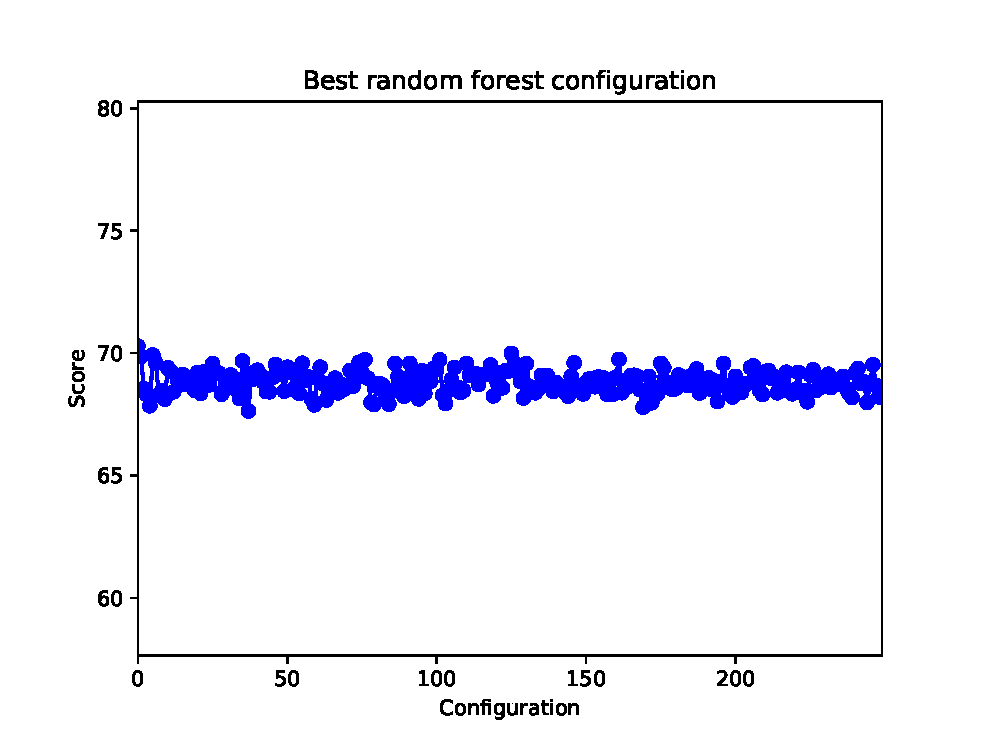
\includegraphics[width=0.8\linewidth]{pictures/random_forest_config.eps}
 \caption{Optimal configuration search for random forest.}
 \label{fig:rf_config}
\end{figure}

The best score registered is $70\%$ with criterion ``entropy'', minimum examples split 2, max features 10 and minimum examples leaf equal to 5.

\subsection{Accuracy testing}

To get an idea about the performances of the newly created random forest instance, an accuracy test is run, with the usual split. The resulted accuracy is equal to $93.946\%$, an optimal result which, if confirmed by cross validation, could classify random forest as one of the best classifiers (the best seen so far) to solve the forest coverage type. Table \ref{tab:rf_test_pr} lists precision, recall and F-measure values for each class. Almost all values for the precision metric are above $90\%$, which means that the classifier is capable of recognizing all the classes really well. Recall values are high too, with class 5 having the lowest registered value of $71\%$.

\begin{table}[H]
\centering
\begin{tabular}{|l|l|l|l|}
\hline
\textbf{Class Index} & \textbf{Precision} & \textbf{Recall} & \textbf{F-Measure}\\\hline
1 & 95.172 & 92.580& 93.858\\\hline
2 & 93.498 & 96.387& 94.921\\\hline
3 & 91.947 & 94.289& 93.104\\\hline
4 & 87.540 & 82.817& 85.113\\\hline
5 & 91.908 & 71.925& 80.698\\\hline
6 & 90.104 & 85.730& 87.862\\\hline
7 & 96.240 & 92.608& 94.389\\\hline
\end{tabular}
\caption{precision, recall and F-measure values using random forest.}
\label{tab:rf_test_pr}
\end{table}

\begin{table}[H]
\centering
\begin{tabular}{|*{7}{c|}r|}
\hline

1 &2 &3 &4 &5 &6 &7 & $\leftarrow$ classified as \\\hline

\cellcolor{black!15}92.58 &7.05 &0.00 &0.00 &0.04 &0.02 &0.31 & 1 \\\hline

2.97 &\cellcolor{black!15}96.39 &0.27 &0.00 &0.17 &0.17 &0.03 & 2 \\\hline

0.02 &2.22 &\cellcolor{black!15}94.29 &0.55 &0.07 &2.86 &0.00 & 3 \\\hline

0.00 &0.00 &14.89 &\cellcolor{black!15}82.82 &0.00 &2.30 &0.00 & 4 \\\hline

1.70 &23.89 &1.89 &0.00 &\cellcolor{black!15}71.93 &0.59 &0.00 & 5 \\\hline

0.14 &4.42 &9.03 &0.65 &0.03 &\cellcolor{black!15}85.73 &0.00 & 6 \\\hline

6.69 &0.69 &0.00 &0.00 &0.01 &0.00 &\cellcolor{black!15}92.61 & 7 \\\hline

\end{tabular}
 \caption{confusion matrix associated to random forest classifier.}
 \label{tab:rf_cm}
\end{table}

Table \ref{tab:rf_cm} shows the confusion matrix. Almost all the instances are concentrated on the diagonal, except for $23.8\%$ of class 5 instances being classified as belonging to class 2 and $14.8\%$ of instances being classified with label 3. 

\subsection{Cross validation}

To find the mean value of the underlying distribution of accuracy associated with the random forest classifier, with a confidence interval of $95\%$, cross validation is run. The resulting sample accuracy mean is $95.166\%$, and with a confidence of $95\%$ the mean of the distribution is inside the confidence interval $95.166 \pm 0.074$. Also, mean precision is equal to $93.578\%$, recall is $90.232\%$ and F-measure is equal to $91.773\%$.  

\begin{figure}[H]
 \centering
 \includegraphics[width=0.8\linewidth]{pictures/random_forest_accuracy_interval.eps}
 \caption{Mean accuracy confidence interval for random forest.}
 \label{fig:rf_accuracy}
\end{figure}

As can be seen in Figure \ref{fig:rf_accuracy}, the confidence interval is really small, so the mean accuracy is expected to be nearly identical to the sample mean. This is because random forest performed very well on each fold, generating points in the Figure \ref{fig:rf_accuracy} that are close to each other.
\begin{table}[H]
\centering
\begin{tabular}{|l|l|l|l|}
\hline
\textbf{Class Index} & \textbf{Precision} & \textbf{Recall} & \textbf{F-Measure}\\\hline
1 & 96.091 & 94.198& 95.135\\\hline
2 & 94.907 & 96.998& 95.941\\\hline
3 & 93.458 & 95.480& 94.457\\\hline
4 & 88.919 & 84.152& 86.392\\\hline
5 & 92.893 & 77.819& 84.673\\\hline
6 & 91.890 & 88.364& 90.080\\\hline
7 & 96.886 & 94.615& 95.734\\\hline
\end{tabular}
 \caption{precision, recall and F-measure values associated to random forest.}
 \label{tab:rf_pr}
\end{table}

Table \ref{tab:rf_pr} shows that precision and recall values for each class are extremely high, even for class 5 where other classifiers have a noticeable drop in performance.
\begin{figure}[H]
 \centering
 \includegraphics[width=0.8\linewidth]{pictures/random_forest_fmeasure.eps}
 \caption{F-measure values resulting from cross validation.}
 \label{fig:rf_fmeasure}
\end{figure}

Finally, Figure \ref{fig:rf_fmeasure} illustrate the F-measure values associated to each class. The plot immediately remarks that random forest, because of its nature (that is, is an ensemble method), is capable of ``memorizing'' particular traits of certain instances that are rare in the dataset (and that other classifiers may lose due to the abundance of other type of instances). In fact, every class presents an high harmonic mean, meaning that random forest is well aware of the existence and nature of that class of instances.

\subsection{Learning curve}

The last part of the experiment on the random forest classifier concerns its ability to improve its performance in predicting instances when presented with a greater number of instances to use as training set. As usual, the dataset is divided in ten parts of different sizes, and the classifier is tested on them. Table \ref{tab:rf_learning} sums up data collected during this test. With the smallest dataset the accuracy registered is $83.7\%$; with the largest the accuracy is equal to $94.1\%$. In other words a $11\%$ increment in performance is registered. Furthermore, as it is clear in Figure \ref{fig:rf_learning}, accuracy grows constantly as the dataset size increments. It can be deduced that random forest performance definitely depends on the dataset size. 

\begin{table}[H]
\centering
\begin{tabular}{|l|l|}
\hline
\textbf{Dataset Size} & \textbf{Accuracy}\\\hline
58102 & 83.710\\\hline
116203 & 87.901\\\hline
174304 & 89.323\\\hline
232405 & 90.657\\\hline
290506 & 91.491\\\hline
348607 & 92.363\\\hline
406708 & 92.724\\\hline
464809 & 93.109\\\hline
522910 & 93.527\\\hline
581011 & 94.162\\\hline
\end{tabular}
\caption{Datasets size and relative accuracies.}
\label{tab:rf_learning}
\end{table}

\begin{figure}[H]
 \centering
 \includegraphics[width=0.8\linewidth]{pictures/random_forest_size_vs_accuracy.eps}
 \caption{Random forest learning curve.}
 \label{fig:rf_learning}
\end{figure}

\section{Models comparison}
In this section data gathered in experiments relative to every tested classifier is used to perform a comparison between them in order to gain insights about which one is more suitable to predict the forest cover type, why, and what are the difference with the other candidates. As first step classifiers' mean accuracies are plotted in Figure \ref{fig:comp_accuracies}.

\begin{figure}[H]
 \centering
 \includegraphics[width=0.8\linewidth]{pictures/comp_accuracies.eps}
 \caption{classifiers' accuracy.}
 \label{fig:comp_accuracies}
\end{figure}

The worst classifier is Gaussian Naive Bayes, with $17.46\%$, that means it is completely incapable of modeling the phenomenon. Next comes Multinomial Naive Bayes, which scores $64.1\%$. An increment in accuracy equal to $46.6\%$, obtained just by switching the underlying distribution of feature values. The Neural Network trained obtains an accuracy of $80\%$, classifying itself as  
a potential solution. Decision Tree has a score of $88.5\%$ but Random Forest is the best classifier with an accuracy of $95.1\%$

In general can we stated that the feature independence assumption is not valid (this is quite obvious, since various features encodes single attributes), and this is why Naive Bayes does not perform well.

Neural network classifier has fairly good precision and recall values (Table \ref{tab:nn_cross_pr}) for the most frequent classes, but experiences a drop in performances on instances belonging to less frequent classes, especially class 5. This may be due to the nature of the training algorithm, since it gives more importance to latest items picked from the training set, and the probability of them to belong to class 1, 2, 3 is (a lot) higher than belonging to the remaining ones (see Figure \ref{fig:class_dist}). 

Decision tree classifier goes a step further gaining a good accuracy value within a tight confidence interval and good F-measure values for each class (Figure \ref{fig:dt_fmeasure}). Decision tree outperforms Neural Networks and Naive Bayes because its structure matches very well the type of features that describe a generic instance of the dataset. Most of the features are binary values and can be interpreted as answer to a ``binary question'' when passing trough an internal node of the tree in order to split the data (in training phase) or to classify an instance.

Finally, Random Forest has on this problem the benefits of the decision tree plus the fact that it has multiple different decision trees, a subset of which potentially focusing on a particular class. This can explain the high accuracy of this classifier and its good performance even on class 5 instances that are the most difficult to recognize.

The last words are on the learning curve of the classifiers. Neural network, decision tree and random forest's accuracy show dependency on the number of samples in the dataset. The dataset is quite large to build a good classifier as it has been seen, but more data could further improve accuracy and make error rate negligible.

In conclusion, this report has seen various classifiers trying to model the forest cover phenomenon. After a series of tests and a comparison Random Forest tool classifies itself as the one to be chosen to solve the problem, especially when class distribution is highly unbalanced.

\end{document}